\section{Methods}
%\IEEEPARstart{T}{his} 
In many cases, the operation provides by a DCEL could involve large spatial datasets.  Our aim is to offer a solution to deal with data volumes that the current sequential solution are unable to process.  In order to reach that goal we are purposing a partition strategy to build a scalable DCEL in a parallel fashion.  

The main idea of the strategy is to split the study area into a number of cells which could be processed independently in a local basis. Let's takes the example of overlay operations over layers of polygons as an example to explains the details. In the sequential approach, the DCEL for each layer will be built and then both will be merged to generate a structure where the operator can be applied.  

Our intention is to create DCELs for each layer in parallel.  The proposal can be summarized in the following steps: (i) Partition the input polygons and build local DCEL representations of them at each partition; (ii) Merge the local DCELs for each layer together locally scaling the processing cost; (iii) Overlay operations will be run over the local merged DCELs to finally be collected back to mix and generate the final answer.  

Figure \ref{fig:overlay_parted} illustrates the proposed partition schema.  We will use a sample of edges from both layers to create a set of cells which will spatially partition the space into disjoint areas.  In the example, a simple grid is used but any spatial index can be applied (in our experiments we use quadtrees for better balance and data distribution).  We will use those cells to clip the input polygons to generate new ones that will lie inside of the boundaries of the cell.  Although it will increase the number of edges and the size of the data, we expect that that the gain during parallel processing will make the addition worthwhile.

\begin{figure}[!ht]
    \centering
    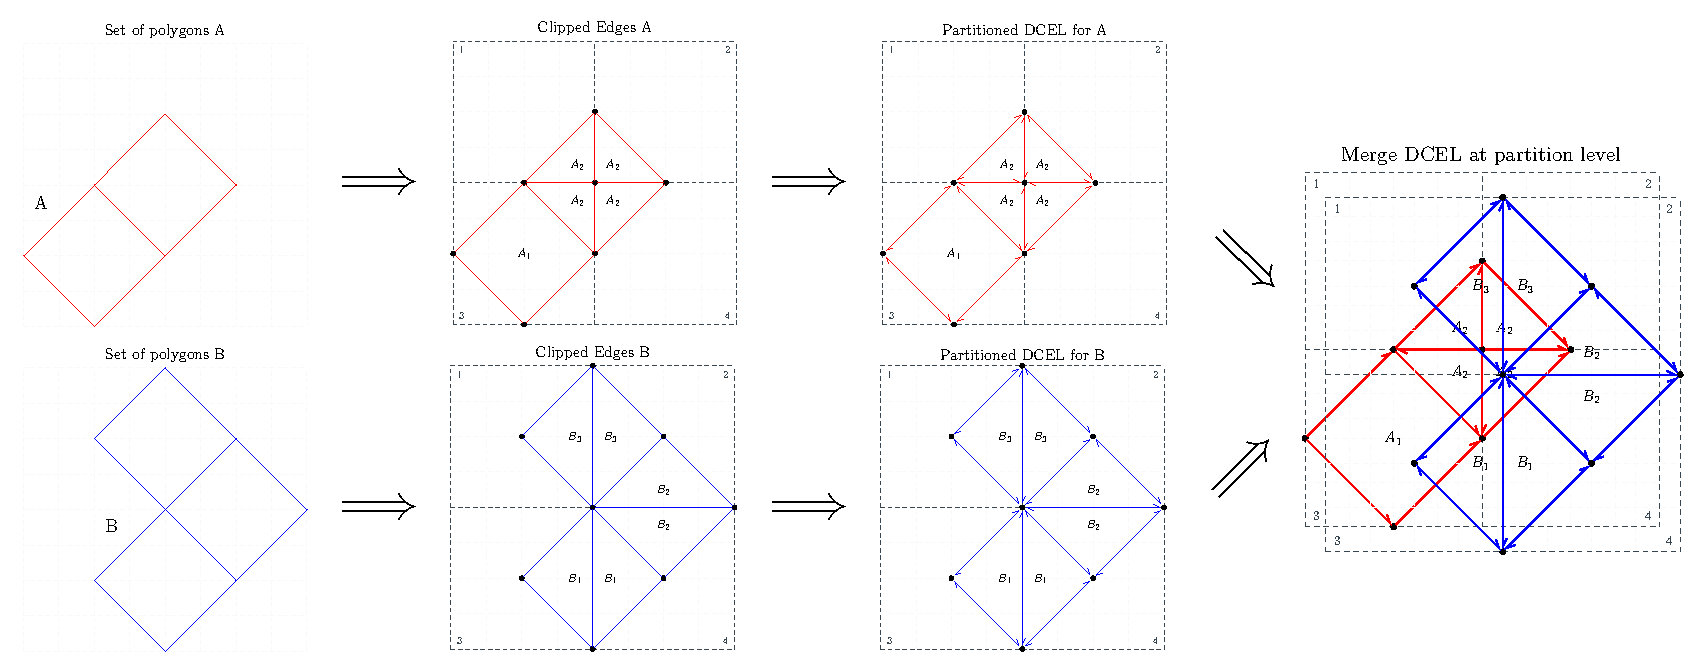
\includegraphics[width=\textwidth]{figures/01-OverlayParted}
    \caption{Partition schema.}\label{fig:overlay_parted}
\end{figure}

Now each cell have the enough data to build a DCEL representation of the new polygons for each layer.  Data for each cell will be marked appropriately and submitted to different nodes to be processed in parallel.  Note that the same partition schema (set of cells) is used in both layers.  That is important due to it allows one-to-one matching between corresponding partitions in both layers.

During the local DCEL construction for individual layers, it is straightforward the connection between the edges inside of each polygon.  From the inputs, it can easily be identified the position of each edge relate to its next and previous edges and to which face's (polygon's) boundary the edge belongs.  Each edge is converted to a half\_edge and their pointers are update accordingly.  However, a query to identify the twin pointer of each half\_edge is still needed given that the input polygons do not provide which polygons are in its neighborhood. The matching is done through a self-join query among the current half\_edges to pair those which share the same vertices in opposite directions.

However, when we pair the partitions from the both layers, we got two local DCELs (each representing the polygons for each layer) and the processing we need now is a merge between both of them.  It requires: (i) Identify the intersection points between the half\_edges of each local DCEL and add them as new vertices; (ii) Split those half\_edges involve in an intersection with a recently added vertex (prune duplicates if needed); (iii) Traverse the list of vertices and update their incident half\_edges list; (iv) Update the pointers for next and previous half\_edges in those affected by the splits; (v) Update the list of faces and their corresponding labels.

Figure \ref{fig:part2} depicts an overview of the process taking as example the polygons and edges of partition 2 of figure \ref{fig:overlay_parted}.  Similarly, figure \ref{fig:merged_dcel} shows the full result of the merged DCEL once all the partitions have processed their corresponding edges. Note that red half\_edges have been introduced artificially by the partition schema but they are marked accordingly to be used in the collect back process when we need to unify the results after the application of the overlay operations.

\begin{figure}[!ht]
    \centering
    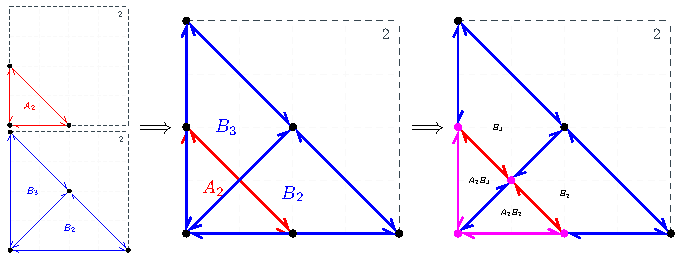
\includegraphics[width=0.75\textwidth]{figures/02-Part2}
    \caption{Merge of local DCEL for partition 2.}\label{fig:part2}
\end{figure}

\begin{figure}[!ht]
    \centering
    \tikzset{    
    barbarrow/.style={ % style that just defines the arrow tip
        %>={Straight Barb[left,length=5pt,width=5pt]},
        >={Triangle[left,length=5pt,width=5pt]},
        double,
        semithick,
        <->
    },
    whites/.style={
        thick, 
        color=white
    }
}
\definecolor{light-gray}{gray}{0.9}
\scalebox{0.9}{
\begin{tikzpicture}
    \tikzstyle{node1}=[draw,scale=0.4,shape=circle,color=black,fill=black]
    \tikzstyle{node2}=[draw,scale=0.4,shape=circle,color=red,fill=red]    
    \draw[color=light-gray, style=dashed] (0,0) grid (8,8);
    \draw[color=red, style=dashed, step=4] (0,0) grid (8,8);
    \node[node1] (A) at (0,2) {};    \node[node1] (C) at (2,0) {};
    \node[node1] (D) at (2,2) {};    \node[node1] (E) at (2,4) {};
    \node[node1] (F) at (2,6) {};    \node[node1] (G) at (3,1) {};
    \node[node1] (H) at (3,3) {};    \node[node1] (I) at (3,5) {};
    \node[node1] (J) at (4,0) {};    \node[node1] (K) at (4,2) {};
    \node[node1] (L) at (4,4) {};    \node[node1] (M) at (4,6) {};
    \node[node1] (N) at (4,8) {};    \node[node1] (O) at (5,3) {};
    \node[node1] (P) at (5,5) {};    \node[node1] (Q) at (6,2) {};
    \node[node1] (R) at (6,4) {};    \node[node1] (S) at (6,6) {};
    \node[node1] (T) at (8,4) {};

    \node at (1,2)      {$A_1$};
    \node at (6.5,4.6)  {$B_2$};
    \node at (6.5,3.4)  {$B_2$};
    \node at (3.4,6.5)  {$B_3$};
    \node at (4.6,6.5)  {$B_3$};
    \node at (4.6,1.5)  {$B_1$};
    \node at (3.6,1)    {$B_1$};
    \node at (3,4.4)    {$A_2$};
    \node at (3,3.6)    {$A_2$};
    \node at (3,2)              {$A_1B_1$};
    \node[scale=0.6] at (3.6,3) {$A_2B_1$};
    \node[scale=0.6] at (4.4,3) {$A_2B_1$};
    \node[scale=0.6] at (5,4.4) {$A_2B_2$};
    \node[scale=0.6] at (5,3.6) {$A_2B_2$};
    \node[scale=0.6] at (3.6,5) {$A_2B_3$};
    \node[scale=0.6] at (4.4,5) {$A_2B_3$};
    
    \draw[barbarrow] (A) -- (C);\draw[barbarrow] (A) -- (E);
    \draw[barbarrow] (C) -- (G);\draw[barbarrow] (D) -- (G);
    \draw[barbarrow] (D) -- (H);\draw[barbarrow] (E) -- (H);
    \draw[barbarrow] (E) -- (I);\draw[barbarrow] (F) -- (I);
    \draw[barbarrow] (F) -- (N);\draw[barbarrow] (G) -- (J);
    \draw[barbarrow] (H) -- (L);\draw[barbarrow] (I) -- (L);
    \draw[barbarrow] (I) -- (M);\draw[barbarrow] (J) -- (Q);
    \draw[barbarrow] (G) -- (K);\draw[barbarrow] (H) -- (K);
    \draw[barbarrow] (K) -- (O);\draw[barbarrow] (L) -- (O);
    \draw[barbarrow] (L) -- (P);\draw[barbarrow] (M) -- (P);
    \draw[barbarrow] (N) -- (S);\draw[barbarrow] (O) -- (Q);
    \draw[barbarrow] (O) -- (R);\draw[barbarrow] (P) -- (R);
    \draw[barbarrow] (P) -- (S);\draw[barbarrow] (Q) -- (T);
    \draw[barbarrow] (S) -- (T);
    
    \draw[whites] (A) -- (C);\draw[whites] (A) -- (E);
    \draw[whites] (C) -- (G);\draw[whites] (D) -- (G);
    \draw[whites] (D) -- (H);\draw[whites] (E) -- (H);
    \draw[whites] (E) -- (I);\draw[whites] (F) -- (I);
    \draw[whites] (F) -- (N);\draw[whites] (G) -- (J);
    \draw[whites] (H) -- (L);\draw[whites] (I) -- (L);
    \draw[whites] (I) -- (M);\draw[whites] (J) -- (Q);
    \draw[whites] (G) -- (K);\draw[whites] (H) -- (K);
    \draw[whites] (K) -- (O);\draw[whites] (L) -- (O);
    \draw[whites] (L) -- (P);\draw[whites] (M) -- (P);
    \draw[whites] (N) -- (S);\draw[whites] (O) -- (Q);
    \draw[whites] (O) -- (R);\draw[whites] (P) -- (R);
    \draw[whites] (P) -- (S);\draw[whites] (Q) -- (T);
    \draw[whites] (S) -- (T);
    
    \draw[barbarrow, color=red] (R) -- (T);\draw[whites] (R) -- (T);
    \draw[barbarrow, color=red] (M) -- (N);\draw[whites] (M) -- (N);
    \draw[barbarrow, color=red] (K) -- (J);\draw[whites] (K) -- (J);
    \draw[barbarrow, color=red] (L) -- (E);\draw[whites] (L) -- (E);
    \draw[barbarrow, color=red] (L) -- (R);\draw[whites] (L) -- (R);
    \draw[barbarrow, color=red] (L) -- (M);\draw[whites] (L) -- (M);
    \draw[barbarrow, color=red] (L) -- (K);\draw[whites] (L) -- (K);
\end{tikzpicture}
}    
    \caption{Result of the merged DCEL.}\label{fig:merged_dcel}
\end{figure}

At this point, we have access to a distributed spatial data structure which collects the individual DCEL representations of the full study area at local basis.  It is easy to see that we can run overlay operations in parallel over the local DCELs and then just collect and merge the results to unify a final answer.  For example, figure \ref{fig:overlay_parted2} illustrates the process to query for the intersection results over the input polygons described in figure \ref{fig:overlay_parted}.

Note that after getting the local results from the local DCELs at each partition, we still need to process those faces which touch the border and can, potentially, have additional sections to be merged in contiguous partitions.  We keep the faces with marked half\_edges for further processing but those ones not involved can be reported immediately.  We use the information of the marked half\_edges to match those that occupy the same place but point on opposite direction.  The faces of those half\_edges are dissolved in one and the involved marked half\_edges are removed. 

\begin{figure}[!ht]
    \centering
    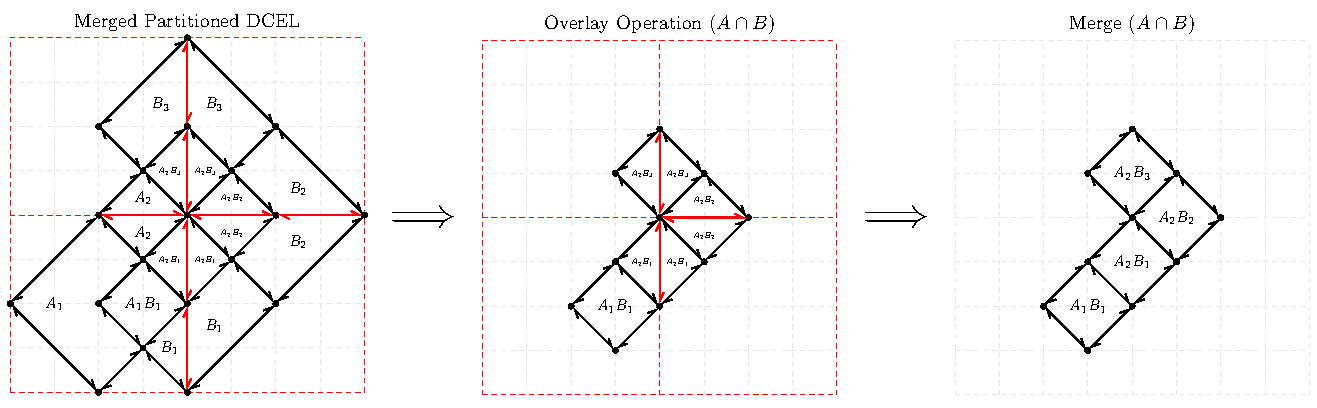
\includegraphics[width=0.75\textwidth]{figures/03-OverlayParted2}
    \caption{Example of an overlay operation querying the distributed DCEL.}\label{fig:overlay_parted2}
\end{figure}

Figure \ref{fig:overlay_operations} shows the results of the five overlay operations supported by the scalable DCEL.  To obtain the results we query locally the DCEL filtering the faces according to the characteristics of its label.  For intersection ($A \cap B$), it filters just faces where its label contains both letters (A and B); On the other hand, for symmetric difference ($A \bigtriangleup B$), it filters faces where its labels contains just one of the letters (A or B).  For the case of difference between the layers ($A \setminus B$ or $B \setminus A$), it filters faces and labels according to the requested letter (either A or B). In the case of union ($A \cup B$), all the faces are retrieved. 

\begin{figure}[!ht]
    \centering
    \tikzset{    
    node1/.style={
        above right
    }
}
\scalebox{0.5}{
    \begin{tikzpicture}
        \node[node1,label={$A \cup B$}]           at (0,0)  {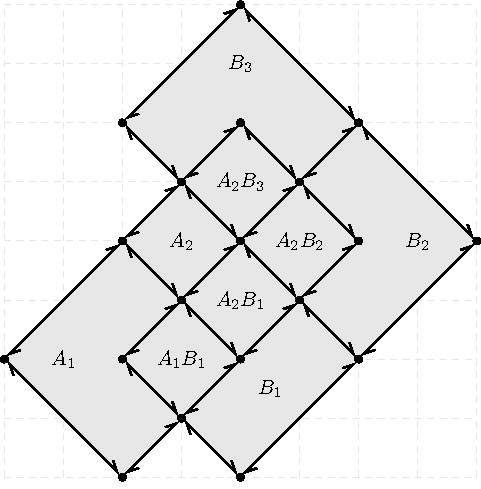
\includegraphics[scale=0.75]{figures/04/DCELUnion}};
        \node[node1,label={$A \cap B$}]           at (7,0)  {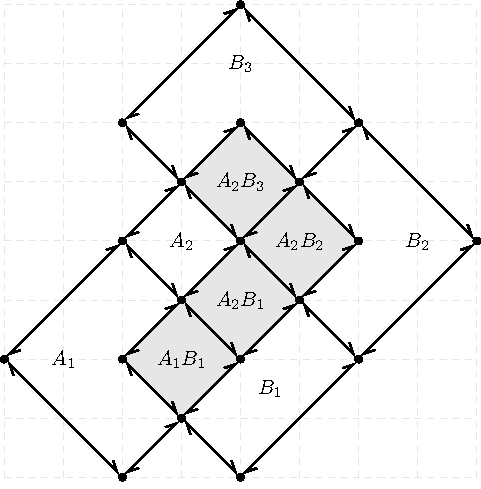
\includegraphics[scale=0.75]{figures/04/DCELIntersection}};
        \node[node1,label={$A \setminus B$}]      at (14,0) {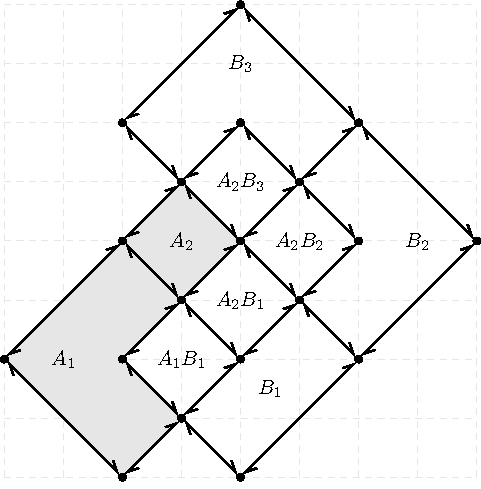
\includegraphics[scale=0.75]{figures/04/DCELDiffA}};
        \node[node1,label={$B \setminus A$}]      at (21,0) {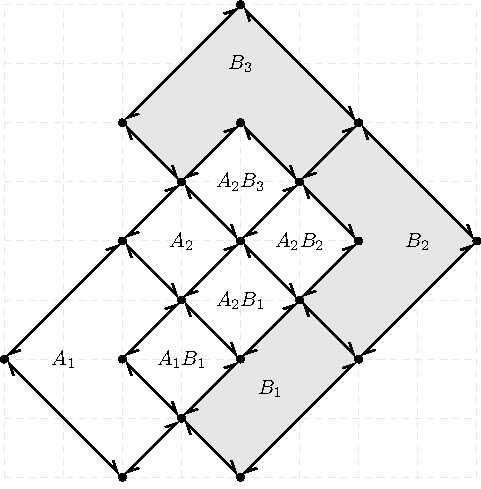
\includegraphics[scale=0.75]{figures/04/DCELDiffB}};
        \node[node1,label={$A \bigtriangleup B$}] at (28,0) {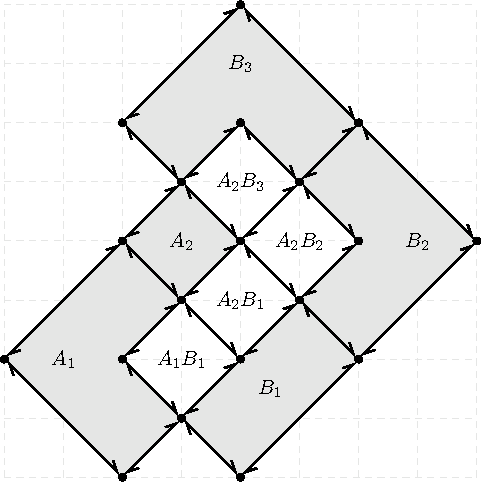
\includegraphics[scale=0.75]{figures/04/DCELDiff}};
    \end{tikzpicture}
}
    \caption{Results of the overlay operations supported by the scalable DCEL.}\label{fig:overlay_operations}
\end{figure}

